\documentclass[10pt,english,aspectratio=169]{beamer}
% Use notes or hide notes or show only notes or handout


\usetheme{default}

\usepackage{xstring}
\usepackage{pgfpages}
%\makeatletter
%\IfSubStr{\@classoptionslist}{handout}
%  {\pgfpagesuselayout{2 on 1}[letterpaper,border shrink=5mm]}
%  {}
%\makeatother

\usepackage{amsmath,amssymb,amsthm}
\usepackage{stmaryrd}
\usepackage{enumerate}
\usepackage{stfloats}
\usepackage{bbm}
\usepackage{pdfpages}
\usepackage{framed}
\usepackage{tabularx}
\usepackage{scalerel}

\usepackage[most]{tcolorbox}
\tcbset{highlight math style={enhanced,
  colframe=white,colback=yellow!15,arc=8pt,boxrule=1pt,
  }}
  
\usepackage{tikz,pgf,pgfplots}
\usepackage{algorithm,algorithmic}
\usepgflibrary{shapes}
\usetikzlibrary{%
  arrows,%
  arrows.meta,
  backgrounds,
  shapes.misc,% wg. rounded rectangle
  shapes.arrows,%
  shapes,%
  calc,%
  chains,%
  matrix,%
  positioning,% wg. " of "
  scopes,%
  decorations.pathmorphing,% /pgf/decoration/random steps | erste Graphik
  shadows,%
  backgrounds,%
  fit,%
  petri,%
  quotes
}

\tikzset{background rectangle/.style={
    fill=white,
  },
  use background/.style={    
    show background rectangle
  }
}

\setbeamersize{text margin left=10mm,text margin right=35mm}

\pgfplotsset{compat=1.12}

%\usetheme{Frankfurt}
%\usecolortheme{ldpc}
\useinnertheme{rounded}
\usecolortheme{whale}
\usecolortheme{orchid}

\newcommand{\ul}[1]{\underline{#1}}
\renewcommand{\Pr}{\mathbb{P}}

%% Setup slides and notes
\makeatletter
\IfSubStr{\@classoptionslist}{notes} { \IfSubStr{\@classoptionslist}{hide} {}{\IfSubStr{\@classoptionslist}{only} {}{\setbeameroption{show notes on second screen=right}}} }{}
\makeatother
%\setbeamertemplate{note page}{\pagecolor{yellow!5}\vfill\insertnote\vfill}

\newcommand{\getpdfpages}[2]{\begingroup
  \setbeamercolor{background canvas}{bg=}
  \addtocounter{framenumber}{1}
  \includepdf[pages={#1},%
  pagecommand={%
    \expandafter\def\expandafter\insertshorttitle\expandafter{%
      \insertshorttitle\hfill\insertframenumber\,/\,\inserttotalframenumber}}%
  ]{#2}
  \endgroup}

\newcommand{\backupbegin}{
   \newcounter{finalframe}
   \setcounter{finalframe}{\value{framenumber}}
}
\newcommand{\backupend}{
   \setcounter{framenumber}{\value{finalframe}}
}

 \setbeamercolor{bibliography entry author}{fg=black}
 \setbeamercolor{bibliography entry title}{fg=black}
 \setbeamercolor{bibliography entry location}{fg=black}
 \setbeamercolor{bibliography entry note}{fg=black}
 
 \setbeamerfont{bibliography item}{size=\footnotesize}
 \setbeamerfont{bibliography entry author}{size=\footnotesize}
 \setbeamerfont{bibliography entry title}{size=\footnotesize}
 \setbeamerfont{bibliography entry location}{size=\footnotesize}
 \setbeamerfont{bibliography entry note}{size=\footnotesize}
 \setbeamertemplate{bibliography item}{\insertbiblabel}
 
\newlength\tikzwidth
\newlength\tikzheight


\newcommand{\mc}[1]{\mathcal{#1}}
\newcommand{\mbb}[1]{\mathbb{#1}}
%\newcommand{\expt}{\mbb{E}}
%\newcommand{\dd}{\mathrm{d}}
\newcommand{\Interior}[1]{\ensuremath{{#1}^{\circ}}}
\newcommand{\Closure}[1]{\ensuremath{\overline{#1}}}
\newcommand{\Complement}[1]{\ensuremath{{#1}^{c}}}

\newcommand{\Expect}{\ensuremath{\mathrm{E}}}
\newcommand{\vecnot}{\underline}
\newcommand{\RealNumbers}{\ensuremath{\mathbb{R}}}
\newcommand{\RationalNumbers}{\mathbb{Q}}
\newcommand{\ComplexNumbers}{\mathbb{C}}
\newcommand{\Real}{\mathrm{Re}}
\newcommand{\Span}{\mathrm{span}}
\newcommand{\Rank}{\mathrm{rank}}
\newcommand{\Nullity}{\mathrm{nullity}}
\newcommand{\Trace}{\mathrm{tr}}
\newcommand{\Diag}{\mathrm{diag}}
\newcommand{\dd}{\mathrm{d}}
\DeclareMathOperator*{\esssup}{ess\,sup}

% Use < , > inner product
\newcommand{\inner}[2]{{\left\langle #1 \mskip2mu , #2 \right\rangle}}
\newcommand{\tinner}[2]{{\langle #1 \mskip1mu , #2 \rangle}}

% Use < | > inner product
%\newcommand{\inner}[2]{{\left\langle #1 \mskip2mu \middle| \mskip2mu #2 \right\rangle}}
%\newcommand{\tinner}[2]{{\langle #1 \mskip1mu | \mskip1mu  #2 \rangle}}




\def\checkmark{\tikz\fill[scale=0.4](0,.35) -- (.25,0) -- (1,.7) -- (.25,.15) -- cycle;}
\def\greencheck{{\color{green}\checkmark}}
\def\scalecheck{\resizebox{\widthof{\checkmark}*\ratio{\widthof{x}}{\widthof{\normalsize x}}}{!}{\checkmark}}
\def\xmark{\tikz [x=1.4ex,y=1.4ex,line width=.2ex, red] \draw (0,0) -- (1,1) (0,1) -- (1,0);}
\def\redx{{\color{red}\xmark}}

\renewcommand{\footnotesep}{-2pt}


\begin{document}

\title{ECE 586: Vector Space Methods \\ Lecture 16 Flip Video: Derivatives in Banach Spaces}
\author{Henry D. Pfister \\ Duke University}
\date{}
%\date{August 20th, 2020}
%\maketitle

\setbeamertemplate{navigation symbols}{}

\begin{frame}[plain]
	\titlepage
	
	\note{
		\vspace{8mm}
		\begin{enumerate}
			\setlength\itemsep{3mm}
			\color{red}
			\item Welcome to the 11th video lecture for ECE 586, Vector Space Methods. \\[2mm]
			Today, we'll finish our discussion of subspaces and bases and then move on to linear transforms.
		\end{enumerate}
	}
\end{frame}

\addtocounter{framenumber}{-1}
\setbeamertemplate{navigation symbols}{\textcolor{blue}{\footnotesize \insertframenumber ~/ \inserttotalframenumber}}



\begin{frame}{Engineering and Optimization}

The foundation of engineering is the ability to use math and physics to \textcolor{blue}{design and optimize complex systems}.

\vspace{4mm}

\textcolor{red}{Computers have now made this possible on an unprecedented scale.}

\vspace{4mm}

Well-known applications include: \vspace{1mm}
\begin{itemize}
\setlength\itemsep{3mm}
\item<1-> Physical Modeling: fitting large physical models (e.g., weather) to huge amounts of collected data

\item<2-> Machine Learning: optimizing non-linear functions (e.g., neural networks) to minimize classification loss on supervised samples

\item<3-> In both cases, optimization benefits from \textcolor{blue}{computing derivatives}

\end{itemize}
\end{frame}

\begin{frame}{Derivatives}

In vector analysis, \textcolor{blue}{derivatives provide local linear approximations}: \vspace{1mm}
\begin{itemize}
\setlength\itemsep{4mm}
\item<1-> For $f\colon \RealNumbers^n \to \RealNumbers^m$ with \textcolor{blue}{Jacobian matrix} $J(\vecnot{x})\in \RealNumbers^{m\times n}$, this gives \vspace{-1mm}
\[ \begingroup \renewcommand*{\arraystretch}{1.35} \!\!\!\!\!\!\! f(\vecnot{x} + \vecnot{h}) \approx f(\vecnot{x}) + J(\vecnot{x}) \vecnot{h}, \;\;\;\;
%\text{where} \;\;
J(\vecnot{x})\triangleq f'(\vecnot{x}) \triangleq  \begin{bmatrix} \frac{\partial  f_1}{\partial  x_1} (\vecnot{x}) & \frac{\partial  f_1}{\partial  x_2} (\vecnot{x}) & \cdots & \frac{\partial  f_1}{\partial  x_n} (\vecnot{x}) \\
\frac{\partial  f_2}{\partial  x_1} (\vecnot{x}) & \frac{\partial  f_2}{\partial  x_2} (\vecnot{x}) & \cdots & \frac{\partial  f_2}{\partial  x_n} (\vecnot{x}) \\
\vdots & \vdots & \ddots & \vdots \\
\frac{\partial  f_m}{\partial  x_1} (\vecnot{x}) & \frac{\partial  f_m}{\partial  x_2} (\vecnot{x}) & \cdots & \frac{\partial  f_m}{\partial  x_n} (\vecnot{x}) \end{bmatrix} \endgroup \]
%where $\vecnot{x},\vecnot{h} \in \mathbb{R}^n$ and $[J(\vecnot{x})]_{ij} = \frac{\partial [f(\vecnot{x})]_i}{\partial x_j} = \lim_{\epsilon \to 0} \frac{[f(\vecnot{x} + \epsilon \vecnot{e}_j) - f(\vecnot{x})]_i}{\epsilon}$

\item<2-> For $f \colon X \to Y$, it is \textcolor{blue}{best to view $f'(x)$ as a linear transform $T \colon X \to Y$} from the domain to codomain.
This transform maps an infinitesimal input perturbation $\vecnot{h}$ to an infinitesimal output perturbation \vspace{-1mm}
$$f'(\vecnot{x})(\vecnot{h}) = T \vecnot{h} = J(\vecnot{x}) \vecnot{h}$$
 
\item<3-> Notice that this definition of the derivative requires a linear structure (to define differences) and a topology (to define convergence) for $X$ and $Y$

%\item<3-> Now, consider the case where $f$ represents that we want to minimize and $m=1$.
%Then, we can decide how to locally adjust the parameter $x$ in order to reduce the value of $f$.

\end{itemize}
\end{frame}

\begin{frame}{Gradient Descent in $\mathbb{R}^n$}

\vspace{15mm}

\hspace*{65mm}
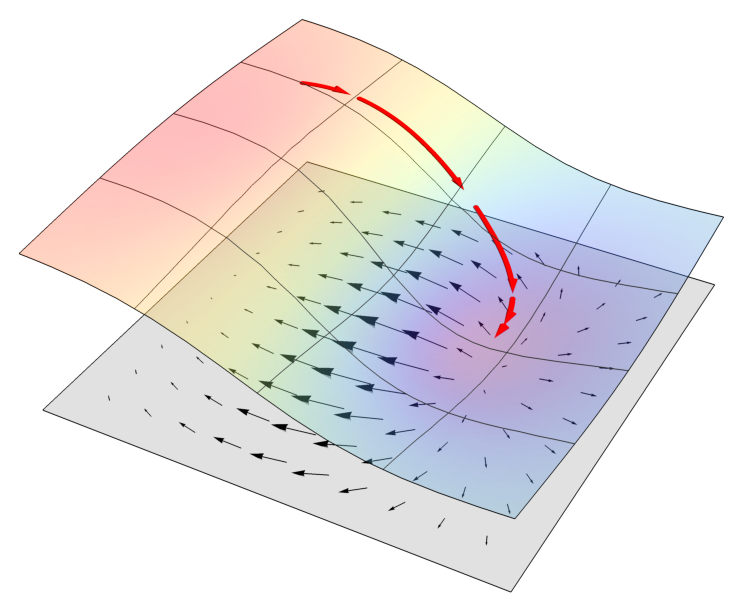
\includegraphics[width=2.5in]{figures/gradient.pdf}
\vspace{-71mm}

\begin{itemize}

\item<1-> Consider a cost function $f\colon \mathbb{R}^n \to \mathbb{R}$ \vspace{1mm}

\begin{itemize}
    \item Can we adjust $\vecnot{x} \in \mathbb{R}^n$ to minimize the cost? \vspace{1mm} 
    \item The \textcolor{blue}{gradient vector} $\nabla f (\vecnot{x}) \triangleq f'(\vecnot{x})^T$ equals \\ the direction of maximum increase \vspace{0mm} \[ \hspace*{-50mm} \nabla f(\vecnot{x}) = \left( \frac{\partial  f}{\partial  x_1} (\vecnot{x}), \, \frac{\partial  f}{\partial  x_2} (\vecnot{x}), \, \cdots, \, \frac{\partial  f}{\partial  x_n} (\vecnot{x}) \right)^T \]

\end{itemize}

\vspace{1mm}

\item<2-> Gradient descent \vspace{1mm}

\begin{itemize}
	\item Discrete time (step size $\delta_n$) \vspace{2mm}
	\[ \hspace*{-50mm} \vecnot{x}_{n+1} = \vecnot{x}_{n}-\delta_n \, \nabla f(\vecnot{x}_{n}) \vspace{1mm} \]
	\item Continuous time: \vspace{2mm} \[ \hspace*{-50mm} \frac{d}{dt} \vecnot{x}(t) = - \nabla f \big( \vecnot{x}(t) \big)  \vspace{1mm} \]
	\item Standard method for training machine learning \\  models like neural networks
\end{itemize}


\end{itemize}

\end{frame}

\begin{frame}{Derivatives in Banach Spaces}

In abstract math, derivatives are usually introduced using Banach spaces: \vspace{1mm}
\begin{itemize}
\setlength\itemsep{3mm}
\item<1-> For a function $f \colon X \rightarrow Y$, the concept of a derivative requires a linear structure (to define differences) and a topology (to define convergence) on both $X$ and $Y$ \vspace{1mm}

\item<2-> If $X=\RealNumbers^n$ and $Y=\RealNumbers^m$, then the derivative of $f$ is a linear transform from $X$ to $Y$ represented by the Jacobian matrix $f'(\vecnot{x}) \in \RealNumbers^{m\times n}$ \vspace{1mm}

\item<3-> Thus, we generally assume that $f \colon X \rightarrow Y$ is a mapping from the Banach space $(X,\|\cdot\|_X)$ to the Banach space $(Y,\|\cdot\|_Y)$ \vspace{1mm}

\item<4-> For directional derivatives, one needs even less structure and it suffices to let $X$ be only a vector space.

\end{itemize}
\end{frame}

\begin{frame}{What is Meant by Differentiable?}

In abstract math, there are many related definitions that are slightly different.
To distinguish between these, one often uses names that are less common in the engineering literature (e.g., Hamel vs.\ Schauder basis).

\vspace{3mm}

\begin{definition}[Differentiable]
Let $f \colon X \rightarrow Y$ be a mapping from a Banach space $(X,\|\cdot\|_X)$ to a Banach space $(Y,\|\cdot\|_Y)$.
Then, $f$ is \textcolor{blue}{Fr\'{e}chet differentiable} at $\vecnot{x}$ if there is a continuous linear transformation $T\colon X \to Y$ satisfying
\begin{equation*} \lim_{\vecnot{h} \to \vecnot{0}} \frac{\left\|f(\vecnot{x}+ \vecnot{h}) - f(\vecnot{x}) - T(\vecnot{h}) \right\|_Y}{\| \vecnot{h} \|_X} = 0,
\end{equation*}
where the limit is with respect to the implied Banach space mapping $X\to \RealNumbers$.
In this case, the \textcolor{blue}{Fr\'{e}chet derivative} $f'(\vecnot{x})$ equals $T$.
\end{definition}
\end{frame}

\begin{frame}{Properties of the Derivative}

A useful property of the derivative is a characterization Lipschitz continuity.

\begin{lemma}
Let $X,Y$ be Banach spaces and $f \colon X \rightarrow Y$ be a function.
If the Fr\'{e}chet derivative $f'(\vecnot{x})$ exists and satisfies $\| f'(\vecnot{x})\|_{\mathrm{op}} \leq L$ for all $\vecnot{x}$ in a convex set $A\subseteq X$, then $f$ is Lipschitz continuous on $A$ with Lipschitz constant $L$.
\end{lemma}

\vspace{4mm}

\uncover<2->{One can also prove a general chain rule for the Fr\'{e}chet derivative.}

\begin{theorem}<2->
Let $X,Y,Z$ be Banach spaces and let $f \colon X \rightarrow Y$ and $g\colon Y \to Z$ be functions.
If $f$ is Fr\'{e}chet differentiable at $\vecnot{x}$ and $g$ is Fr\'{e}chet differentiable at $\vecnot{y}=f(\vecnot{x})$, then $(g \circ f) (\vecnot{x}) = g(f(\vecnot{x}))$ is Fr\'{e}chet differentiable at $\vecnot{x}$ with derivative $g'(f(\vecnot{x}))\circ f'(\vecnot{x})$.
\end{theorem}


\end{frame}

\begin{frame}{Directional Derivatives}

Directional derivatives differ from standard derivatives in that the perturbation vector is provided as a argument.
For $f\colon \RealNumbers^n \to \RealNumbers^m$, this means that the directional derivative is not a linear transform but just a vector in $\mathbb{R}^m$.

\vspace{2mm}

\begin{definition}[Directional Derivative]<1->
Let $f \colon X \rightarrow Y$ map vector space $X$ to a Banach space $(Y,\|\cdot\|)$.
Then, if it exists, the \textcolor{blue}{G\^{a}teaux differential} of $f$ at  $\vecnot{x}$ in direction $\vecnot{h}$ is given by \vspace{-1.5mm}
\[ \delta f (\vecnot{x};\vecnot{h}) \triangleq \lim_{t \to 0} \frac{f(\vecnot{x}+t \vecnot{h}) - f(\vecnot{x})}{t}. \]
%where the limit is with respect to the implied mapping from $\RealNumbers$ to $Y$.
\end{definition}

\begin{example}<2->
Consider $X\!=\!Y\!=\!\mathbb{R}^2$ and $f(\vecnot{x})\! =\! (x_1 x_2,x_1+x_2^2)$.
For $\vecnot{x}\!=\!(1,1)$, $\vecnot{h}\!=\!(1,2)$: \vspace{-2.5mm}
\[ \delta f ( \vecnot{x},\vecnot{h} ) = \frac{d}{dt} ((1+t)(1+2t),(1+t)+(1+2t)^2) \Big|_{t=0} = (3,5). \]
\end{example}


\end{frame}

\begin{frame}{Properties of the Directional Derivative}

\begin{lemma}<1->
Let $Y=\RealNumbers$ and suppose that $\delta f (\vecnot{x};\vecnot{h})$ exists and is negative for some $f$, $\vecnot{x}$, and $\vecnot{h}$.  Then, there exists $t_0 > 0$ such that, for all $t\in(0,t_0)$, one has \vspace{-2mm}
\[ f(\vecnot{x}+t \vecnot{h}) < f (\vecnot{x}). \]
\end{lemma}

\visible<1->{Proof in live session.}

\vspace{5mm}

\begin{definition}<2->
Let $f \colon X \rightarrow Y$ be a mapping from a vector space $X$ to a Banach space $(Y,\|\cdot\|)$.
Then, $f$ is \textcolor{blue}{G\^{a}teaux differentiable} at $\vecnot{x}$ if the G\^{a}teaux differential $\delta f (\vecnot{x};\vecnot{h})$ exists for all $\vecnot{h} \in X$ and is a continuous linear function of $\vecnot{h}$.
\end{definition}

\end{frame}


\begin{frame}{On the Gradient in Hilbert Space}

For $f\colon \RealNumbers^n \to \RealNumbers^m$ with $m=1$, the Jacobian is related to the \textcolor{blue}{gradient}
\[ \nabla f(\vecnot{x}) \triangleq f'(\vecnot{x})^T  = \left[ \begin{array}{cccc} \frac{\partial  f}{\partial  x_1} (\vecnot{x}) & \frac{\partial  f}{\partial  x_2} (\vecnot{x}) & \cdots & \frac{\partial  f}{\partial  x_n} (\vecnot{x}) \end{array} \right]^T. \]
It is worth noting that the orientation of the gradient vector (i.e., row versus column vector) is sometimes defined differently.
This is because derivatives can be understood as linear transforms and either orientation can be used to define the correct linear transform. 

\begin{example}
Let $X$ be a Hilbert space over $\RealNumbers$ and $f\colon X \to \RealNumbers$ be a real functional.
If the Fr\'{e}chet derivative $f'(\vecnot{x})$ exists, then it is a continuous linear functional on $X$.
Thus, the Riesz representation theorem guarantees that there is a vector $\vecnot{u} \in X$ such that
$ f'(\vecnot{x})(\vecnot{h}) = \tinner{\vecnot{h} }{ \vecnot{u} } $ for all $\vecnot{h}\in X$.
This vector is called the gradient $\nabla f(\vecnot{x})$ and it follows that \vspace{-1mm}
$$ f'(\vecnot{x})(\vecnot{h}) = \tinner{\vecnot{h} }{ \nabla f (\vecnot{x}) } \text{ for all } \vecnot{h}\in X. $$
\end{example}

\end{frame}



\begin{frame}{Gradient Descent}

\begin{itemize}
\setlength\itemsep{1.5mm}
\item<1-> Gradient descent subtracts the gradient $\nabla f(\vecnot{x})$ from an element of $X\!\!\!$

\item<2-> For a Banach space, the derivative is a linear functional mapping $X$ to $\RealNumbers$!

\item<3-> How can one add a linear mapping to $X$?

\item<4-> In Hilbert space, the Riesz representation theorem states every linear functional is represented by the inner product with a fixed vector

\item<5-> Thus, the gradient $\nabla f (\vecnot{x}) \in X$ is defined as the representative vector
\end{itemize}

\begin{definition}[Gradient Descent]<6->
Let $f \colon X \rightarrow \RealNumbers$ be a mapping from a Hilbert space $X$ to the standard Banach space of real numbers.
Starting from $\vecnot{x}_1 \in X$, \textcolor{blue}{gradient descent} defines the sequence \vspace{-1mm}
\[ \vecnot{x}_{n+1} = \vecnot{x}_n - \delta_n \nabla f(\vecnot{x}_n), \]
where $\delta_n$ is the step size for the $n$-th step.
% and the gradient $\nabla f (\vecnot{x})$ is uniquely defined by \vspace{-1.5mm}
%\[\tinner{ \vecnot{h} }{ \nabla f(\vecnot{x}) } = f'(\vecnot{x})(\vecnot{h}) \text{ for all } \vecnot{h} \in X. \]
\end{definition}

\end{frame}

\begin{frame} \frametitle{Bounds for a Lipschitz Gradient}

\begin{lemma}
Let $f \colon X \rightarrow \RealNumbers$ map the Hilbert space $X$ to the real numbers.
If $\nabla f(\vecnot{x})$ exists and satisfies $ \| \nabla f(\vecnot{y}) - \nabla f(\vecnot{x}) \| \leq L \| \vecnot{y} - \vecnot{x} \|$, then \vspace{-3mm}
\[ \big| f(\vecnot{y}) - f(\vecnot{x}) - \tinner{\vecnot{y}-\vecnot{x} }{ \nabla f (\vecnot{x}) } \big| \leq \frac{1}{2} L \| \vecnot{y}-\vecnot{x} \|^2. \]
\end{lemma}
\vspace{-1mm}
\begin{proof}<2->
Let $\vecnot{h} = \vecnot{y}-\vecnot{x}$ and $\phi(t) = f(\vecnot{x} + t \vecnot{h})$. Then, $\phi'(t) = \tinner{ \vecnot{h} }{ \nabla f(\vecnot{x} + t \vecnot{h}) }$ and \vspace{-2.5mm}
\begin{align*}
\big| f(\vecnot{y}) -  f(\vecnot{x}) - \tinner{ \vecnot{h} }{ \nabla f(\vecnot{x}) } \big|  &= \left| \scaleobj{0.85}{\int_{0}^1} \left( \phi'(t) - \phi'(0) \right) \mathrm{d}t \right| \\
\uncover<3->{&=  \left| \scaleobj{0.85}{\int_{0}^1} \tinner{ \vecnot{h} }{ \nabla f(\vecnot{x} + t \vecnot{h}) - \nabla f(\vecnot{x}) } \, \mathrm{d}t \right| \\}
\uncover<4->{&\leq \left| \scaleobj{0.85}{\int_{0}^1}  \| \vecnot{h} \| \, \| \nabla f(\vecnot{x} + t \vecnot{h}) - \nabla f(\vecnot{x}) \| \, \mathrm{d}t \right| \\}
\uncover<5->{&\leq \scaleobj{0.85}{\int_{0}^1} \|\vecnot{h} \| L \| t \vecnot{h} \| \, \mathrm{d}t = \frac{1}{2} L \| \vecnot{h} \|^2. }
\end{align*}
\vspace{-6.5mm}
\end{proof}

\end{frame}

\begin{frame} \frametitle{Next Steps}

\begin{itemize}
\setlength\itemsep{5mm}
\item To continue studying after this video -- \vspace{2mm}

\begin{itemize}
 \setlength\itemsep{3mm}
 \item Try the required reading: Course Notes EF 5.1
 %item Or the recommended reading: LADR 6AB
 \item Also, look at the gradient descent problem in Assignment 6
\end{itemize}
\end{itemize}

\note{
	\vspace{8mm}
	\begin{enumerate}
		\setlength\itemsep{3mm}
		\color{red}
		\item Here are some options to continue learning this material. (read) \\ [2mm]  That's it for today.  So, I'll see you next time.
	\end{enumerate}
}

\end{frame}


\end{document}

\backupbegin

%\begin{frame}
%\frametitle{Backup Slides}
%\begin{itemize}
%\item Slide numbers not included in denominator!
%\end{itemize}
%\end{frame}

%\begin{frame}[allowframebreaks]
%\frametitle{References}
%\bibliographystyle{alpha}
%\footnotesize
%\bibliography{IEEEabrv,WCLabrv,WCLbib,WCLnewbib}
%\end{frame}

\backupend

\end{document}
